\subsection{Graphit}
Die Graphitschicht konnte magnetisch auf der Probenhalterung angebracht werden. Die Vorbereitungen f�r die Graphitmessung dauerten nicht lange, da nach wenigen Versuchen eine funktionsf�hige Pt-Ir-Spitze angefertigt werden konnte. F�r die Anfertigung der Pt-Ir-Spitze standen Isopropanol, Reinigungst�cher, eine Pinzette und eine Zange zu halten des Drahtes. Um den Pt-Ir-Draht anzuspitzen, stand uns ein Seitenschneider zur Verf�gung, mit dem der Draht angeschnitten wurde, sodass durch darauffolgendes kr�ftiges Ziehen eine (idealerweise) einatomige Spitze erzeugt werden konnte.
Nachdem eine passende Pt-Ir-Spitze hergestellt werden konnte, wurde mit dem RTM ein Bereich von 600nm im "`Topographie"'-Modus (CC) abgerastert.
Die dazu ben�tigten Einstellungen konnten mit dem Programm f�r das RTM eingestellt werden und sind in Tabelle \ref{tab:para_topo_graph} dargestellt.
\begin{table}[H]
\centering
\caption{Parameter zur Topographiemessung (CC-Mode)}
\begin{tabular}{c|c}
Variable & Wert\\
\hline Set point & \SI{1}{nA}\\
P-gain & 1000\\
I-gain & 1700\\
Tip-voltage & \SI{50}{mV}\\
\end{tabular}
\label{tab:para_topo_graph}
\end{table}
Die Topographiemessung �ber \SI{600}{nm} ist in Abbildung \ref{fig:topo_graph_600nm} dargestellt.
\begin{figure}[H]
\centering
\includegraphics[scale = 0.75,clip = true, trim = 0cm 6.2cm 0cm 0cm]{ausschnitt_600}
\caption{ \SI{600}{nm} Bild im Topographie/CC-Modus }
\label{fig:topo_graph_600nm}
\end{figure}
\subsubsection{Rauheit}
Die Rauheit der Graphitschicht konnte mit der Software f�r das RTM bestimmt werden, nachdem die Graphitschicht im CC-Modus mit der Spitze des RTM abgerastert wurde. Die Verkippung wurde bestimmt und grob bis auf \SI{0,2}{\degree} korrigiert. Das Fenster Topography-Scan ist f�r die Messung nicht wichtig, da es die Oberfl�chenbeschaffenheit ausschlie�lich auf H�he des schwarzen Pfeils angibt. In Abbildung \ref{fig:lin_rau_graph} ist die Messung zur Bestimmung der mittleren Linienrauheit dargestellt.
\begin{figure}[H]
\centering
\includegraphics[scale = 0.75]{snipping_122_linienrauheit}
\caption{ Mittlere Linienrauheit von Graphit entlang der abgebildeten Linie \\ ($R_a = \SI{7,0159}{pm}$ und $R_q = \SI{9,1550}{pm}$) }
\label{fig:lin_rau_graph}
\end{figure}
Ebenso wurde die mittlere Fl�chenrauheit der Graphitprobe bestimmt, welche in Abbildung \ref{fig:flae_rau_graph} dargestellt ist.
\begin{figure}[H]
\centering
\includegraphics[scale = 0.75]{snipping_122_flaechenrauheit}
\caption{ Mittlere Fl�chenrauheit von Graphit f�r die Fl�che im Quadrat \\ ($S_a = \SI{10,471}{pm}$ und $S_q = \SI{13,100}{pm}$) }
\label{fig:flae_rau_graph}
\end{figure}
Man sieht, dass die mittlere Fl�chenrauheit gr��er als die mittlere Linienrauheit ist, wobei der Anteil der arithmetischen Rauheit an der quadratischen Rauheit bei beiden Messungen in etwa gleich gro� ist ($\frac{R_a}{R_q} = 0,78 = 78 \%$ und $\frac{S_a}{S_q} = 0,80 = 80 \%$). F�r die Linienrauheit wurde eine m�glichst glatte Linie gew�hlt, wodurch der Unterschied zur quadratischen Rauheit begr�ndet werden kann. Insgesammt f�llt auf, dass die Oberfl�chenrauheit von HOP-Graphit relativ gering ist. Die �hnlchkeit von Linienrauheit und Fl�chenrauheit sprechen bei dieser Oberfl�che f�r eine gute Messung. 
\subsubsection{Gitterstruktur und Elektronendichteverteilung}

In diesem Abschnitt soll die  Elektronendichteverteilung und die Gitterstruktur des Graphit untersucht werden. Daf�r wurde ein kleiner Bereich herangezoomt, damit die atomare Struktur sichtbar wird. Es wurde ein Bereich von 3 x 3 nm verwendet, der m�glichst glatt erscheint. Die Verkippung der Probe wurde korrigiert, die Aufnahme ist in Abbildung \ref{fig:graphit_atomstruktur} zu sehen.

\begin{figure}[H]
\begin{subfigure}[t]{0.49\textwidth}
\includegraphics[scale = 0.7]{graphit_3nm_nanostruktur_oberflaeche.png}
\caption{Oberfl�che der Graphitprobe bei atomarer Aufl�sung. Es l�sst sich die hexagonale atomstruktur erkennen.}
\label{subfig:graphit_atomstruktur_1}
\end{subfigure}
\hspace{0.02\textwidth}
\begin{subfigure}[t]{0.49\textwidth}
\includegraphics[scale = 0.7]{graphit_3nm_nanostruktur_topographie.png}
\caption{Beispielhafter topologischer Verlauf, entlang der x-Achse}
\label{subfig:graphit_atomstruktur_2}
\end{subfigure}
\caption{Aufnahme der Oberfl�chen von Graphit in einem Bereich von 3 x 3 nm. Die H�hendifferenz liegt im Bereich von \SI{1,5}{\angstrom} }
\label{fig:graphit_atomstruktur}
\end{figure}

Um die Gitterstruktur noch besser sehen zu k�nnen, wird die Oberfl�che noch im Constant Hight Mode gescant. Daf�r werden der P$_{gain}$ auf 0V und der I$_{gain}$ auf 4V eingestellt. F�r den Scan wurde eine Fl�chen von 1,1 x 1,1 nm gew�hlt. Die Aufnahme, mit eingezeichneter hexagonaler Struktur ist in Abbildung \ref{fig:graphit_1_1_nm_struktur} zu sehen. Die Aufnahme wurde geschert, damit die Gitterstruktur besser zu erkennen ist.

\begin{figure}[H]
\centering
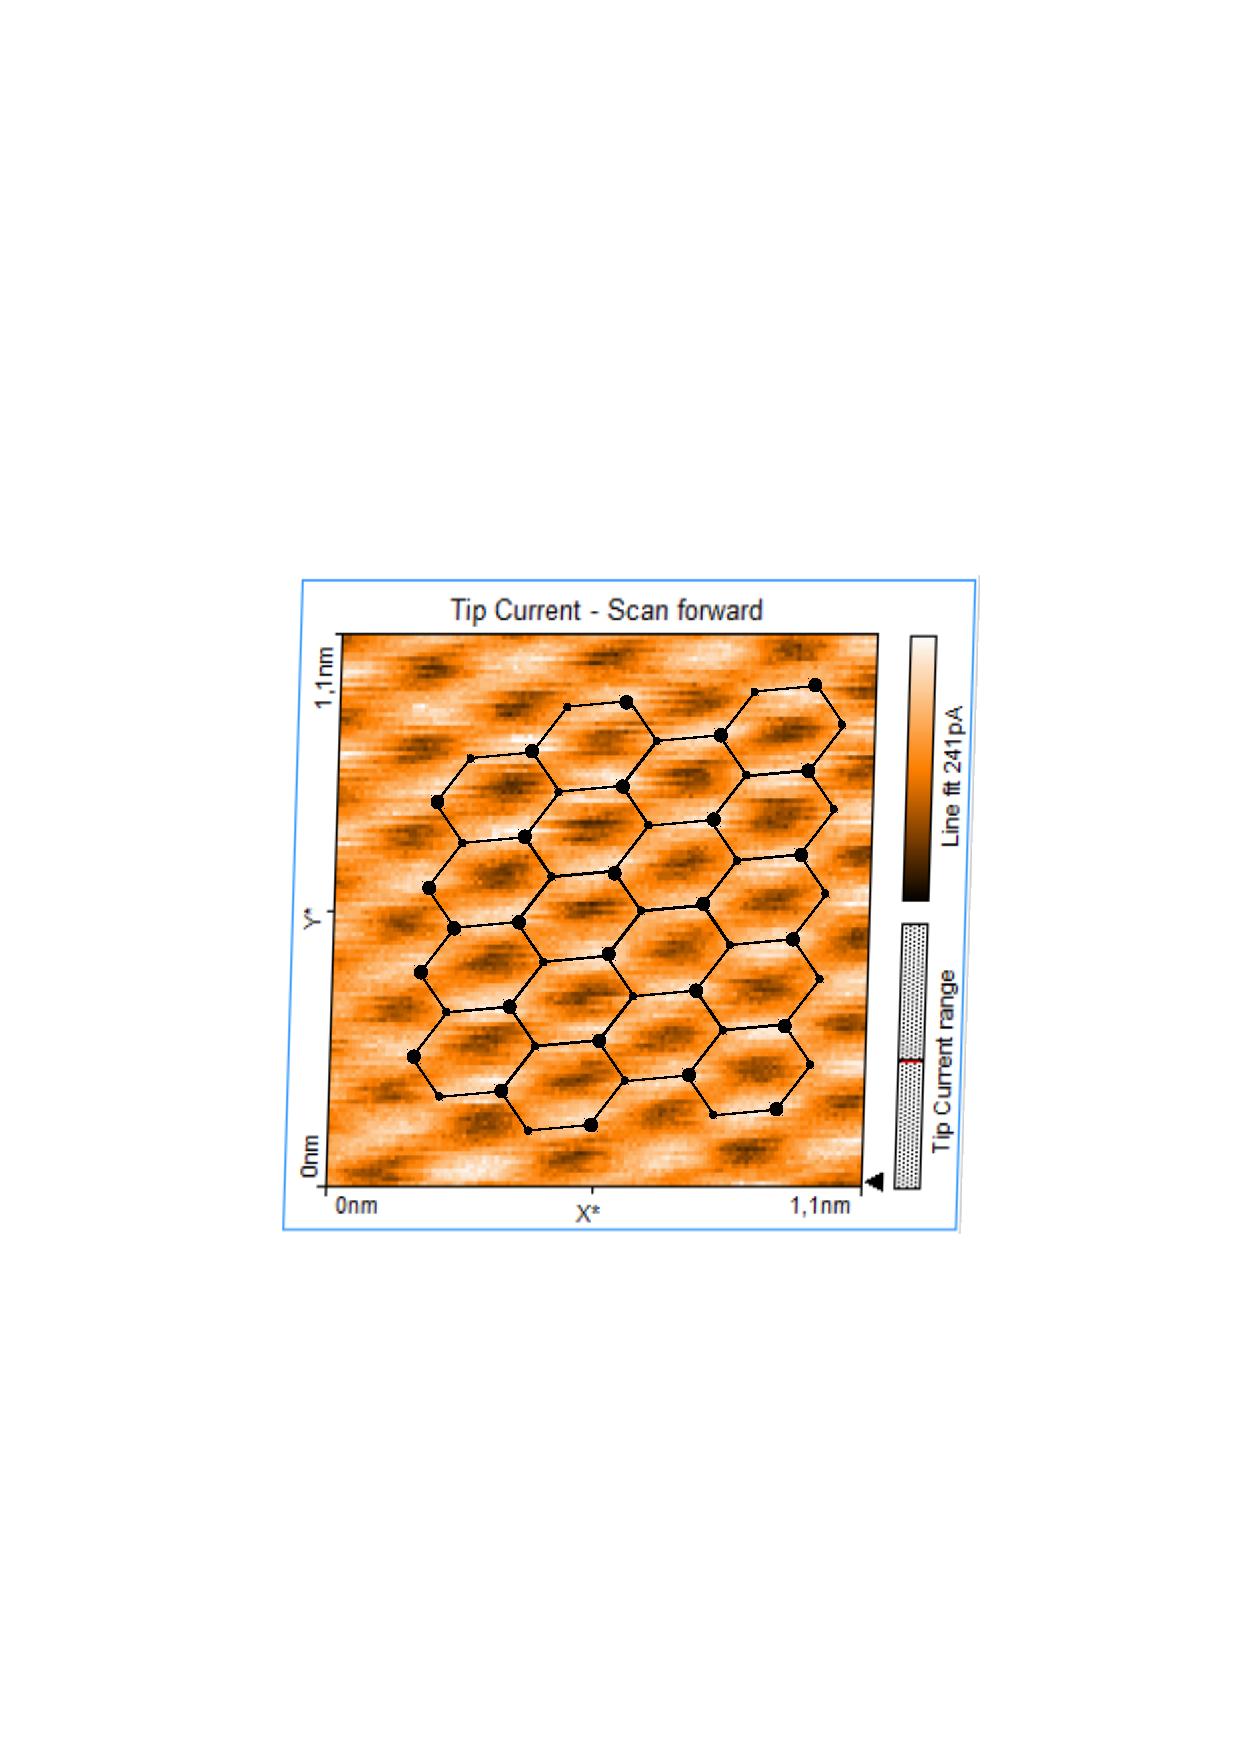
\includegraphics[trim = 10mm 90mm 10mm 90mm, clip, scale = 0.75]{graphit_1,1nm_CHM_struktur.jpg}
\caption{Aufnahme der Oberfl�che im Bereich von 1 x 1 nm. Zur Veranschaulichung wurde die Gitterstruktur eingezeichnet.}
\label{fig:graphit_1_1_nm_struktur}
\end{figure}

Abbildung \ref{fig:graphit_1_1_nm_struktur} ist so zu interpretieren, dass an den hellen Stellen die Gitteratome ohne Verbindungen zur darunterliegenden Schicht liegen, daher liegen die Elektronen direkt am Atom an und es wird ein h�herer Tunnelstrom gemessen. An den orangen Stellen befinden sich die Atome mit einer Verbindung zur darunterliegenden Schicht, wodurch der Tunnelstrom geringer wird. Die schwarzen Bereich entsprechen den mitten der Hexagonalenstruktur, bei welchen die das n�chste Atom erst in der darunter liegenden Schicht liegt und somit der Tunnelstrom sehr gering ist.
\subsubsection{Mittlerer Atomabstand}
\begin{figure}[H]
\centering
\includegraphics[scale = 0.75]{snipping_122_linienrauheit}
\caption{ Mittlere Linienrauheit von Graphit entlang der abgebildeten Linie \\ ($R_a = \SI{7,0159}{pm}$ und $R_q = \SI{9,1550}{pm}$) }
\label{fig:mittlere_Atomabstand}
\end{figure}